
We construct the index structure on features. Our index structure is a chain hashing structure. For a give data point to be inserted in to the structure, for each of it features, we hash the feature and insert the reference to the data point in the chain. In our current implementation we have used a hash table of size 785985, and hence we do not have any collisions. The hash table is maintained as a binary search tree. This structure results in a chain of maximum length 264016.\\

\section{Point Query}

Point query operation can be very effectively 
implemented in the inverted index structure. To perform this operation we maintain a list of candidate nodes, which needs to be explored sequentially. Our aim is to prune the candidate list as much as possible. This pruning is done by the following observation.\\
Given a point $p$ we look at all its features, and find the list of all nodes associated with the features. It is a straight forward observation that $p$ is present in the dataset only if, it is in the intersection of all the associated point list. This reduces our candidate list to a size, atleast as small as the smallest list, among all the features present in $p$ (which in our case is on an average only 271).\\

\section{Range Query and K-nn}
Range query and K-nn are much more complicated queries, when compared to a point query. The candidate set in this case is much more diverse and distributed. For example the candidate set for a Range query will be the union of all the point lists associated with the features of $p$, which is the worst case is of the order of $N$. We try to prune this by observing that the minimum number of features in a point is 7, hence we can remove the top 6 features from the index with out affecting the accuracy of searching. But this pruning does not result in any improvement in performance. We shall discuss this further the sections below.\\

\section{Baseline technique}
 Given a query q, which has features $f_1, f_2,...f_{N_q}$ we take a union of all compounds present in atleast one of these features and then proceed with a linear search. This is described in detail below.

\begin{enumerate}
	\item We keep a hash table where every feature has a pointer to the set of points which contains that feature itself.
	\item Let the feature $f_1$ of query q be present in the points $p_1,p_2,...p_M$. Let this set be $S_1$.
	\item We take a union of all such sets $S_1, S_2,...S_{N_q}$ defined as the set $S_q$
	\item We do a linear search on the compounds present in this set.
	\item The answer are the subset of points of the set $S_q$ which fall within threshold t of the query.	 
\end{enumerate}


\begin{figure}[ht]	
\centering
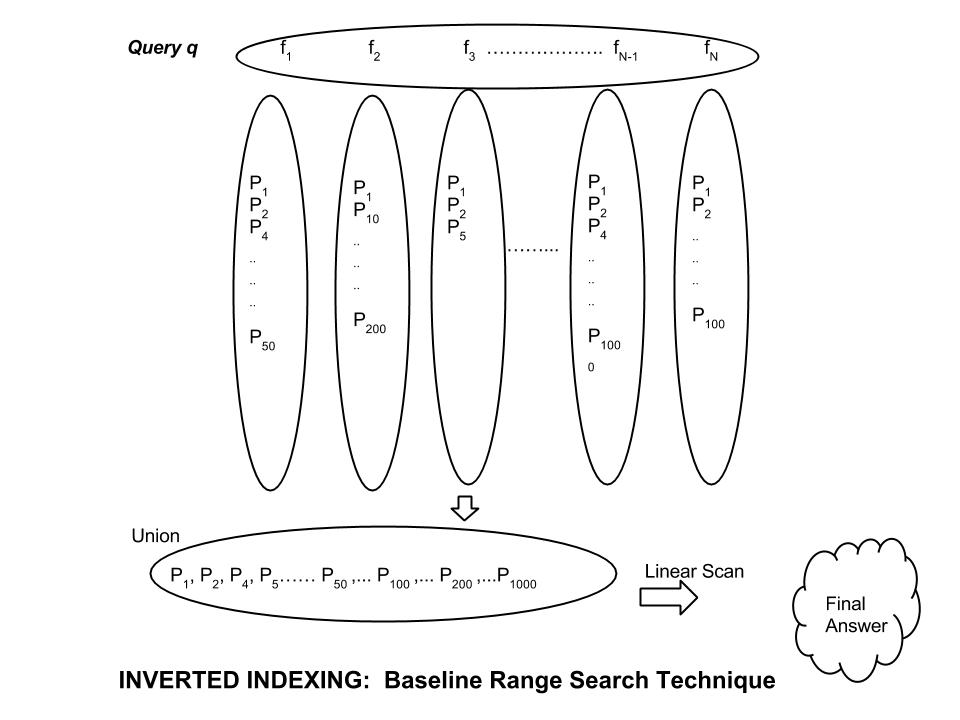
\includegraphics[width=1 \columnwidth]{img/image0c.jpg}
\caption{Inverted Indexing: Procedure Diagram}
\label{fig: invert}
\end{figure}




\section{Pruning Features}
 We use a greedy technique to prune features i.e. prune out features whose points are guaranteed to lie outside distance threshold.
 
\begin{enumerate}
	\item We sort the features of the query q, $f_1,f_2,...f_{N_q}$ in descending order of popularity i.e. the feature present in most of the points is at the start.
	
	\item We prune this feature if the maximum similarity value is less than the minimum required similarity threshold.
	
	\item Consider feature $f_1$. Let's say we want to prune this feature. We are concerned with points having this feature but not having any of the other features of the query point. 
	
	\item Let us assume binary fingerprints for simplicity. The maximum similarity such a point can have with the query point is $\frac{1}{N_q - 1 + V_{f_1}}$ where $N_q$ is the number of features in query q and $V_{f_1}$ is the minimum number of features present among all points having the feature $f_1$
	
	\item Hence if  distance threshold is t and the following holds
	\[\frac{1}{N_q - 1 + V_{f_1}}  < 1-t\]
we can prune the feature $f_1$		
	
	\item We continue a greedy approach, where we consider the next feature $f_2$ and try to prune both the features $f_1$ and $f_2$ together.
	
	\item Hence if till the $i^{th}$ feature is considered, if j features have been pruned, we can prune the $i^{th}$ feature as well if the following holds
	\[\frac{j+1}{N_q - 1 + min(V_{f_i}, minimum~set~J~value)} < 1-t \] where  \textit{minimum~set~J~value} is the minimum number of features present in any of the compounds of the features pruned till now.
	
	\item We can extend this to non binary fingerprints as well.
	
\end{enumerate}
